\documentclass[11pt]{article}
\usepackage[T1]{fontenc}
\usepackage[utf8]{inputenc}
\usepackage{lmodern}
\usepackage[a4paper,margin=2.4cm,headheight=14pt]{geometry}
\usepackage{microtype}
\usepackage{amsmath,amssymb}
\usepackage{graphicx}
\usepackage{booktabs,tabularx,array,longtable}
\usepackage[font=small,labelfont=bf]{caption}
\usepackage{xcolor}
\usepackage{pdflscape}
\usepackage{float}
\usepackage{listings}
\usepackage{upquote}
\usepackage{fancyhdr}
\usepackage[numbers,sort&compress]{natbib}
\usepackage[colorlinks=true,linkcolor=blue!50!black,citecolor=blue!50!black,urlcolor=blue!50!black]{hyperref}
\usepackage{bookmark}

\graphicspath{{figures/}{../article/assets/}}
\newcommand{\Records}{100,017}
\newcommand{\Components}{33,575}
\newcommand{\MotherFamilies}{46,613}
\newcommand{\OverlapShare}{79.3}
\newcommand{\ICC}{0.495}
\newcommand{\LargestComponent}{14,101}
\newcommand{\LargestShare}{14.1}
\newcommand{\LargestMean}{6.59}
\newcommand{\AllMean}{5.74}
\newcommand{\RandTrain}{70,011}
\newcommand{\RandVal}{15,003}
\newcommand{\RandTest}{15,003}
\newcommand{\GrpTrain}{69,996}
\newcommand{\GrpVal}{15,017}
\newcommand{\GrpTest}{15,004}
\newcommand{\RandBase}{0.095}
\newcommand{\GrpBase}{0.055}
\newcommand{\RandCut}{7.360}
\newcommand{\GrpCut}{7.402}
\newcommand{\RandComponents}{9,640}
\newcommand{\GrpComponents}{6,002}
\newcommand{\Boot}{2,000}
\newcommand{\BootSeed}{7}
\newcommand{\EmbedSeconds}{134.8}
\newcommand{\EmbedRSS}{1.76}
\newcommand{\MLMAcc}{0.416}
\newcommand{\MajorityBase}{0.329}
\newcommand{\UTRLMParams}{1,208,043}
\newcommand{\PosCacheGB}{1.28}
\newcommand{\RunSeconds}{3,417}
\newcommand{\RunMinutes}{56.9}
\newcommand{\StepSeconds}{3,415.2}
\newcommand{\ErrOverTwo}{289}
\newcommand{\ErrOverTwoReads}{485}
\newcommand{\MedianReads}{616}

\makeatletter\let\inputtab\@@input\makeatother % expandable input for table bodies

\newcommand{\m}[1]{\texttt{#1}}
% Estimate with 95% interval; \stackedci switches to a two-line cell for wide tables.
\newcommand{\ci}[3]{#1 [#2, #3]}
\newcommand{\twoline}[2]{\begin{tabular}[t]{@{}r@{}}#1\\#2\end{tabular}}
\newcommand{\stackedci}{\renewcommand{\ci}[3]{\begin{tabular}[t]{@{}l@{}}##1\\ {}[##2, ##3]\end{tabular}}}
\newcolumntype{L}{>{\raggedright\arraybackslash}X}
\renewcommand{\arraystretch}{1.12}
\setlength{\emergencystretch}{2em}
% Let floats sit closer to their first reference.
\renewcommand{\topfraction}{0.9}\renewcommand{\bottomfraction}{0.8}\renewcommand{\textfraction}{0.07}
\renewcommand{\floatpagefraction}{0.75}\setcounter{totalnumber}{5}\setcounter{topnumber}{3}
\urlstyle{same}
\makeatletter
\g@addto@macro{\UrlBreaks}{\do\a\do\b\do\c\do\d\do\e\do\f\do\g\do\h\do\i\do\j\do\k\do\l\do\m\do\n\do\o\do\p\do\q\do\r\do\s\do\t\do\u\do\v\do\w\do\x\do\y\do\z\do\A\do\B\do\C\do\D\do\E\do\F\do\G\do\H\do\I\do\J\do\K\do\L\do\M\do\N\do\O\do\P\do\Q\do\R\do\S\do\T\do\U\do\V\do\W\do\X\do\Y\do\Z\do\0\do\1\do\2\do\3\do\4\do\5\do\6\do\7\do\8\do\9}
\makeatother
\renewcommand{\bibfont}{\small\raggedright}

\lstset{basicstyle=\ttfamily\footnotesize,columns=fullflexible,keepspaces=true,breaklines=true,
  frame=single,framerule=0.3pt,rulecolor=\color{black!40},xleftmargin=2pt,xrightmargin=2pt,
  showstringspaces=false,upquote=true}

\pagestyle{fancy}
\fancyhf{}
\fancyhead[L]{\footnotesize Choosing a model for 5$'$UTR translation experiments}
\fancyhead[R]{\footnotesize Historical results; independent reproduction pending}
\fancyfoot[C]{\footnotesize \thepage}
\renewcommand{\headrulewidth}{0.3pt}

\hypersetup{pdftitle={Cheap features, a small CNN or frozen UTR-LM? An exploratory comparison for predicting 5' UTR mean ribosome load},
  pdfsubject={Manuscript reporting existing computational results; independent reproduction pending},
  pdfkeywords={5' UTR, mean ribosome load, MPRA, CNN, UTR-LM, RNA language model, benchmark}}

% Supplement S1: embed the byte-identical original article in the PDF (pdfTeX primitives).
\immediate\pdfobj stream attr {/Type /EmbeddedFile /Subtype /text#2Fplain} file {../article/published-original.md}
\edef\origobj{\the\pdflastobj}
\immediate\pdfobj {<< /Type /Filespec /F (S1-published-original.md) /UF (S1-published-original.md) /Desc (Supplement S1: original published article, byte-identical copy) /EF << /F \origobj\space 0 R >> >>}
\edef\origspec{\the\pdflastobj}
\pdfnames {/EmbeddedFiles << /Names [(S1-published-original.md) \origspec\space 0 R] >>}

\begin{document}

\begin{center}
{\LARGE\bfseries Cheap features, a small CNN or frozen UTR-LM?\\[2pt]
An exploratory comparison for predicting\\[2pt] 5$'$UTR mean ribosome load\par}
\vspace{0.8em}
{\large Study repository \texttt{rewire-bio/utr-model-selection}\par}
{\small Author list to be confirmed by the study owner. Drafted with AI assistance; see Section~\ref{sec:disclosure}.\par}
\vspace{0.6em}
{\small Original analysis: 30 September 2026. Manuscript compiled from the archived results: October 2026.\par}
\end{center}

\vspace{0.4em}
\noindent\fbox{\begin{minipage}{\dimexpr\linewidth-2\fboxsep-2\fboxrule\relax}
\small\textbf{Status of this manuscript.} This is a manuscript reporting \emph{existing} computational
results. Every number comes from the companion run executed on 30 September 2026 (archived as
\texttt{downloads/\allowbreak utr-baselines-results.zip}) or from the cited literature; values were extracted and
formatted from the archived outputs, and nothing was recomputed for this manuscript. A fresh, independent
reproduction is \textbf{pending}; the repository's reproduction protocol is an unapproved, unconfigured
scaffold and has not been executed. No result here carries a verified or approved status. All results are
exploratory: both test sets had prior exposure, and the assay is a single unreplicated measurement.
\end{minipage}}

\begin{abstract}
\noindent Laboratories that measure 5$'$UTR libraries by polysome profiling want to predict mean ribosome
load (MRL) for sequences they have not made. We compared ridge regression on cheap sequence features, a
small convolutional neural network (CNN) trained from scratch, and a frozen RNA language model (UTR-LM,
checkpoint \texttt{ESM2\_1.4\_five\_species}) with three trained heads, on the \Records{} designed 5$'$UTRs
of Sample et al.\ (2019), under a protocol registered before any new method was scored. On a grouped split
that keeps families of related sequences (shared parent or identical 20-nt substring) on one side of the
train/test boundary, the one-hot CNN had test MSE 0.560 MRL$^2$ against 0.776 for the best cheap baseline, a
reduction of $+0.216$ [$+0.176$, $+0.252$] (95\% cluster-bootstrap interval), which meets the prespecified
0.10~MRL$^2$ practical threshold. For picking the top 1\% (150) of 15,004 test sequences, the CNN found 86
high-MRL sequences and the cheap baseline 83; the precision difference, $+0.020$ [$-0.088$, $+0.132$], was not
supported, and the interval is too wide to show equivalence. Frozen UTR-LM embeddings were worse than cheap
features with a ridge head on both splits, and as CNN input made no supported difference from one-hot input
on the grouped split ($-0.010$ [$-0.034$, $+0.016$]); on a random split in which 79.3\% of test records had a relative in training they lowered
MSE by $+0.021$, below the threshold, and lowered precision. The results are exploratory: one unreplicated
assay in HEK293T cells, about 70,000 training labels, one frozen checkpoint and one laptop. The endpoint is
ribosome loading on an eGFP reporter, not protein output or endogenous translation. All values are existing results
from a 30 September 2026 run; independent reproduction is pending.
\end{abstract}

\tableofcontents
\clearpage

%======================================================================
\section{Introduction}\label{sec:intro}
A laboratory with a 5$'$UTR reporter library and measured mean ribosome load (MRL, the average number of
ribosomes on each mRNA molecule) often wants to predict MRL for sequences it has not made yet, either to
estimate values or to choose a small set of candidates for follow-up. We consider three options: regression on cheap, interpretable sequence features; a small convolutional network trained on the
library's own labels, in the style of Optimus 5-Prime~\citep{sample2019}; and a pretrained RNA language model
whose representation is fed to a trained head~\citep{chu2024utrlm,shi2025mrnabench}. The last option adds an
embedding step and a dependency on pretrained weights; the question is whether it improves accuracy here.

We compared these options on the designed library of Sample et al.~\citep{sample2019}, processed by
mRNABench~\citep{shi2025mrnabench}, under a protocol fixed before any new method was scored on a test set.
Two questions are distinguished: whether a method predicts MRL values more accurately (mean squared error),
and whether it puts more high-MRL sequences into a fixed top-1\% pick list (precision at 1\% capacity). Two
splits are also distinguished, because related sequences in this library otherwise straddle the train/test
boundary. The contributions are (i) a paired, cluster-bootstrapped comparison of ten methods on a random and a
grouped split with prespecified practical thresholds; (ii) a separation of accuracy gains from pick-list
gains; (iii) a documented accelerator divergence for the language-model embeddings; and (iv) a runnable
companion and results archive behind every number. This comparison is between workflows, not matched
architectures, and every result is exploratory.

%======================================================================
\section{Background and related work}\label{sec:background}

\subsection{The assay}
In the Sample et al.\ assay, in vitro transcribed (IVT) reporter mRNAs are transfected into cells, the lysate
is separated on a sucrose gradient into fractions carrying different numbers of ribosomes, and each fraction is
sequenced. For each 5$'$UTR, MRL is the sum over fractions of its relative read count in each fraction multiplied
by that fraction's ribosome number~\citep{sample2019} (Figure~\ref{fig:assay}). MRL leaves out the ribosome-free
mRNA fraction, so a high-MRL sequence may still have a large untranslated fraction~\citep{castillohair2024}.

\begin{figure}[tp]
\centering
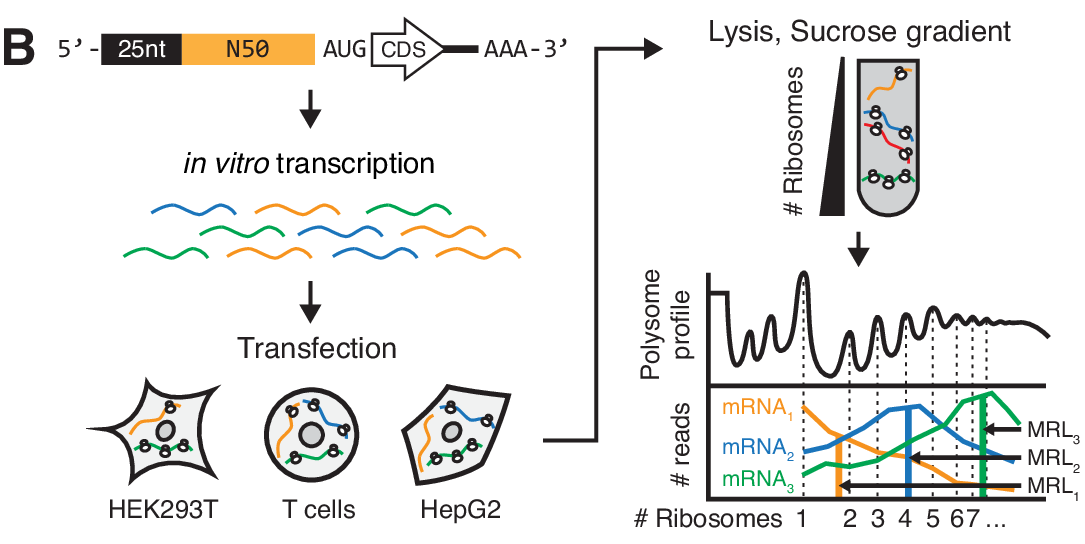
\includegraphics[width=0.85\linewidth]{06-castillo-hair-fig1b-polysome-mpra-schematic.png}
\caption{\textbf{How a polysome-profiling reporter assay turns reads across ribosome fractions into MRL.}
Reporter mRNAs with a fixed 25-nt segment and a variable 50-nt 5$'$UTR are transfected into cells, separated on
a sucrose gradient, and read counts across ribosome fractions give MRL. This panel shows a 2024 library with the
same 25\,nt + 50\,nt construct, not the 2019 data used here. Adapted (cropped) from Castillo-Hair et al.\ 2024,
Fig.~1b~\citep{castillohair2024}, CC~BY~4.0.}
\label{fig:assay}
\end{figure}

\subsection{\texorpdfstring{Models of 5$'$UTR translation}{Models of 5' UTR translation}}
Sample et al.\ trained a CNN (Optimus 5-Prime) on MPRA data and reported variant effects as squared Pearson
correlations of log changes~\citep{sample2019}. UTR-LM~\citep{chu2024utrlm,utrlm_repo} pretrains an ESM2-style
model on 5$'$UTRs and, by default, fine-tunes it on downstream labels; in the authors' ablation on a random
50-nt library with a rank split, a frozen model with a trained MLP head reached Spearman 0.6 against 0.962 fully
fine-tuned~\citep{chu2024supp}. mRNABench~\citep{shi2025mrnabench,mrnabench_code} benchmarks linear probes on
frozen embeddings from many RNA models, and showed that probes and the $k$-mer baseline lost much of their
random-split Pearson correlation when one Kozak/uAUG combination was held out (Figure~\ref{fig:mrnabench}).
In its appendix table the $k$-mer baseline lost 0.34 in Pearson correlation and a probe on \m{utrlm-mrl} lost
0.33, while another UTR-LM variant, \m{utrlm-te-el}, lost 0.17. The figure shows one point per model family,
and its \m{utrlm} point (about 0.56 to 0.39) matches \m{utrlm-te-el}. Karollus et al.~\citep{karollus2021} found
that MPRA-trained MRL models correlate only weakly with endogenous translation measurements.

\begin{figure}[tp]
\centering
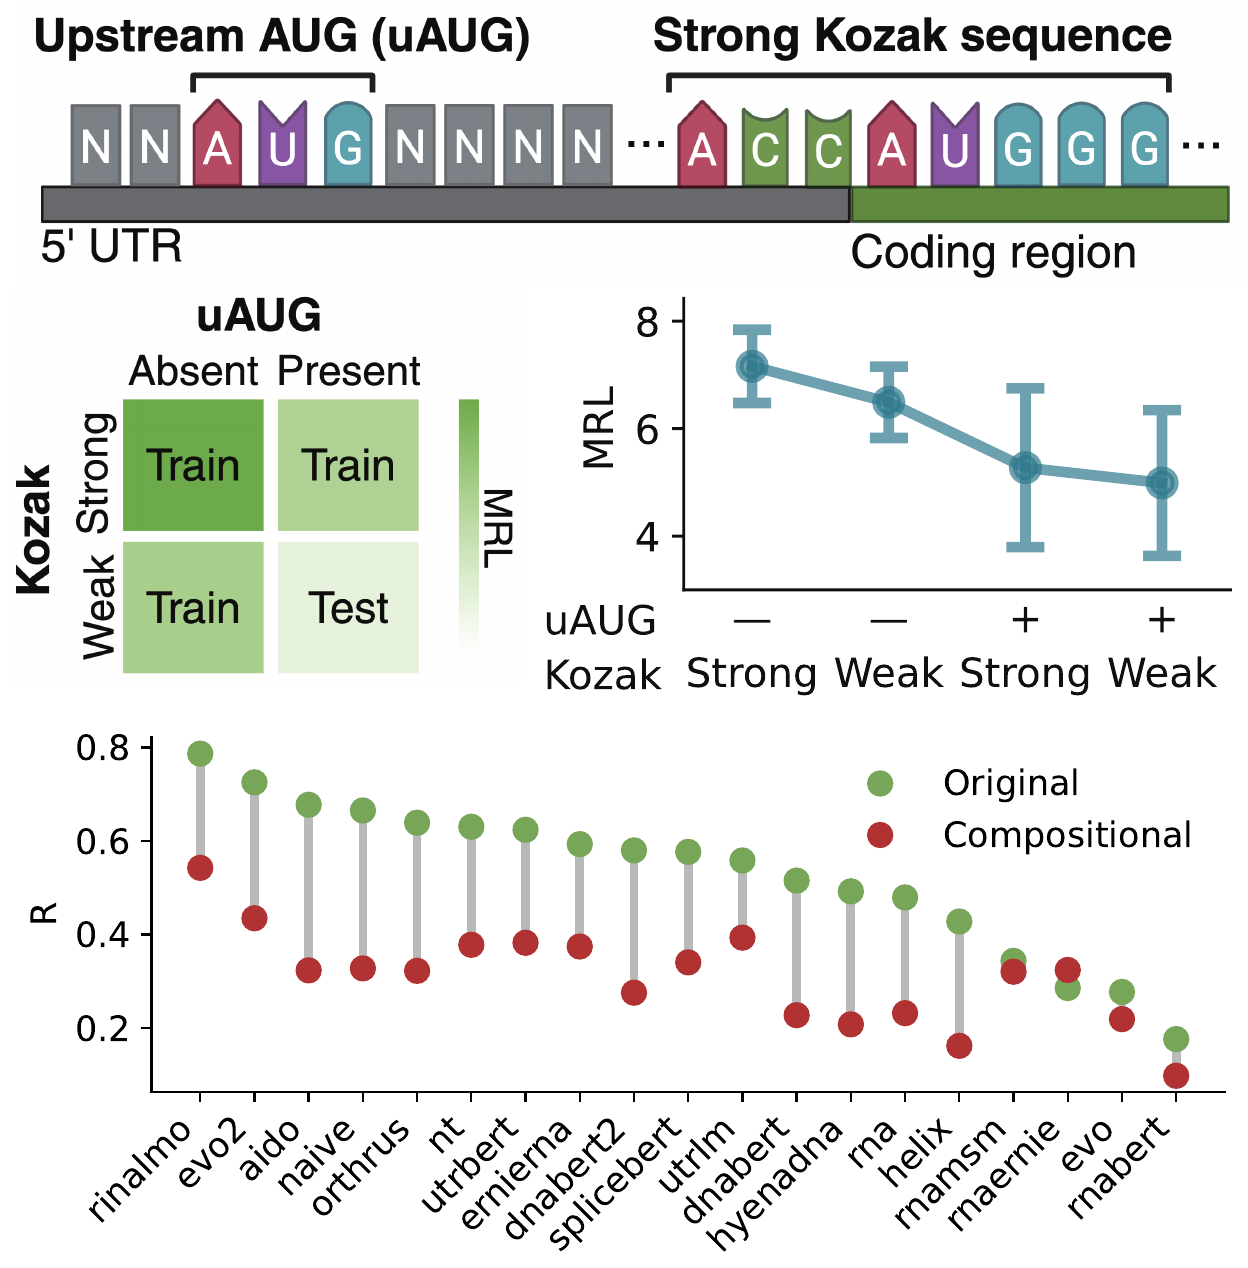
\includegraphics[width=0.62\linewidth]{01-mrnabench-fig7-compositional-split-mrl.png}
\caption{\textbf{Random versus compositional split in mRNABench.} Linear probes on frozen embeddings, and the
$k$-mer baseline, lost much of their random-split Pearson $r$ when one Kozak/uAUG combination was held out;
the supervised CNN is not shown. From Shi et al.\ 2025 (mRNABench), Fig.~7~\citep{shi2025mrnabench},
CC~BY~4.0; cropped.}
\label{fig:mrnabench}
\end{figure}

%======================================================================
\clearpage
\section{Materials and methods}\label{sec:methods}
The protocol (\texttt{utr-mrl-designed-choice-v1}, \texttt{companion/PROTOCOL.md}) was registered on 30
September 2026 at 08:56:32Z, amended once at 09:00:14Z before any test scoring (example rule only), and followed
by nine dated reporting clarifications written after scoring; none changes a method, prediction, threshold or
verdict. Its registered and amended texts are archived with their SHA-256 digests.

\subsection{Data}\label{sec:data}
Each designed-library record is a 25-nt defined leader, a 50-nt insert and the eGFP coding sequence, measured in
HEK293T cells 12 hours after transfection (GEO GSM3130443~\citep{geo_gse114002}). The inserts include 50-nt
fragments of 35,212 human 5$'$UTRs, 3,577 ClinVar variants, genetic-algorithm designs and step-wise evolution
trajectories in which every intermediate was synthesised (80 trajectories, 7,526 UTRs). The \m{mcherry}
sub-library label records design origin: the whole designed library was cloned into the same eGFP vector. Two
of the 13 labels, \m{sergii\_utrs} and \m{egfp\_poor\_performers}, have no documented definition. The library was
measured once, with no duplicate (GEO GSE114002), so there is no replicate-based ceiling on achievable accuracy;
the sources do not state its RNA chemistry.

Processed records come from the mRNABench Hugging Face dataset~\citep{hf_mrlsample} (file \m{mrl-sample-\allowbreak designed.parquet}, revision \m{ef67f7c}); metadata (sub-library, parent \m{mother} sequence, read count) come from GEO and are joined
one to one on the insert, with the GEO MRL required to equal the processed target exactly for all \Records{}
records (maximum difference 0.0). Only the insert varies: the other 805\,nt of each 855-nt processed record are
identical in all records. A replay of an earlier full-sequence composition control from
rewire-benchmarks~\citep{rb_ca73fa4} therefore gives near-identical predictions to insert-only composition
(maximum difference below 0.001 MRL; test MSE 1.914 on the random split). Every method below uses the insert alone.
Appendix Table~\ref{tab:composition} gives the sub-library counts.

\subsection{Splits}\label{sec:splits}
\paragraph{Random split.} The random split (called \m{historical} in the code) is mRNABench's seed-2541 random
split (\RandTrain{} / \RandVal{} / \RandTest{} records), reconstructed from source row order and checked
against its published SHA-256. Its test set had already been used for two published controls, so results on it
are not a fresh test. It also mixes relatives, such as trajectory intermediates and ClinVar variants, with their
source sequences. Linking records that share a GEO parent sequence or any identical 20-nt substring gives
\Components{} families. In the random split, \OverlapShare\% of test records had a relative in training, and
training labels had a within-family intraclass correlation of \ICC.

\paragraph{Grouped split.} The grouped split assigns whole families to training, validation or test
(\GrpTrain{} / \GrpVal{} / \GrpTest{} records). It was registered before scoring, but whole-dataset label
summaries by sub-library had been viewed, so it is not an untouched cohort either. Families holding more than 1\%
of records go to training, and one does: \LargestComponent{} records (\LargestShare\%), 98\% genetic-algorithm
designs, mean MRL \LargestMean{} against \AllMean{} overall. The remaining families are shuffled (seed 20260930)
and assigned to test until it reaches 15\% of records, then to validation (Appendix~\ref{app:code}). The grouped
test set therefore has no \m{step\_random\_to\_best\_no\_uatgs} records, fewer other genetic-algorithm designs, and
a high-MRL rate of \GrpBase{} against \RandBase{}. It is a defined transfer test to sequences with no shared parent
or 20-nt substring in training, not a leakage-free estimate for every designed sequence. Methods should be
compared within a split; the two test sets differ in overlap, composition and base rate.

\subsection{Methods compared}\label{sec:models}
\paragraph{Cheap ridge baselines.} Ridge regression on nucleotide composition (A/C/G/T and GC fractions); counts of
all 1- to 3-mers (84 features); position-specific one-hot (200 features); annotation features computed from the
insert and the known reporter context (upstream AUGs [uAUGs] and their frame, uAUG--stop pairs, stop codons,
Kozak context); and \m{cheap\_combined}, which concatenates the last three. Features are standardised on training
data and the penalty is chosen from $\{10^{-3}, \dots, 10^{4}\}$ by validation MSE. The reference is the cheap
model with the lowest validation MSE: \m{cheap\_combined} on both splits.

\paragraph{Supervised CNN.} An Optimus 5-Prime-style network (three convolutional layers of 120 width-8 filters,
a 40-unit dense layer, dropout 0.2) trained from scratch on one-hot inserts with Adam (learning rate $10^{-3}$,
batch 128, at most 20 epochs, early stopping after 3 epochs without validation improvement). Seeds 0, 1 and 2 were
trained; headline numbers use seed 0, fixed in advance.

\paragraph{Frozen UTR-LM.} The \m{ESM2\_1.4\_five\_species} checkpoint from the UTR-LM repository at
\m{b77b589}~\citep{utrlm_repo} (6 layers, 128 dimensions, \UTRLMParams{} parameters). Its final-layer insert
embeddings fed three heads: ridge on their mean, ridge on all 50 positions (6,400 features), and a CNN head with the
one-hot CNN's layer design. The CNNs take 4 and 128 input channels, so their parameter counts differ: this compares
workflows, not matched architectures. ``Frozen'' means the language model's weights stay fixed and only the head
learns; ``fine-tuned'', the UTR-LM authors' default, means those weights are also updated. Nothing here was
fine-tuned.

The case for this checkpoint is documentary. The UTR-LM paper~\citep{chu2024utrlm} describes a baseline pretrained
only by masked-nucleotide prediction on unlabelled Ensembl 5$'$UTRs from five species, and
\m{ESM2\_1.4\_five\_species} is the only pretrained file whose name carries no token for the Cao et al.\ endogenous
data, a downstream library, structure or free energy. It also loads strictly into plain ESM2. No text names the file
and no sequence-overlap audit was run; human 5$'$UTR fragments in this library may appear, unlabelled, in that
corpus. The \m{FS4.x} checkpoints and MultiMolecule \m{utrlm-mrl}~\citep{multimolecule_utrlm} (used by mRNABench) were
excluded because Sample et al.\ random-library sequences were in their pretraining; the sources do not show that they
saw MRL labels. The chosen model beat the commonest base at masked-nucleotide prediction (\MLMAcc{} against
\MajorityBase), which confirms it loaded and runs, nothing more. Embeddings were computed on CPU
(Section~\ref{sec:device}). Hyperparameters for every method were chosen on validation data, and each method was
scored on the test set once.

Orthrus~\citep{orthrus} was considered and excluded: its pinned \m{mamba-ssm==1.2.0.post1}
dependency~\citep{mamba_ssm} failed to build without CUDA, and it was trained on full mature RNAs. That says nothing
about its accuracy. The failed installation logs are archived.

\subsection{Metrics}\label{sec:metrics}
\textbf{MSE} is the mean squared difference between predicted and measured MRL, in MRL$^2$; lower is better.
Predicting the training mean gives 2.224 on the grouped test set. \textbf{R$^2$} is the coefficient of
determination, $1 - \mathrm{SSE}/\mathrm{SST}$ with SST about the test mean; zero matches predicting the test mean.
It is not the squared Pearson correlation that Sample et al.\ report as $r^2$.

\textbf{Precision at 1\% capacity} matches a follow-up budget. A record is high-MRL if its measured MRL is at or
above the 90th percentile of that split's training labels (\GrpCut{} on the grouped split, \RandCut{} on the random
split). Precision is the high-MRL fraction of the $k = 150$ top-ranked test records (1\%), with ties broken by lower
source index as a fixed convention. Chance is the test high-MRL rate: \GrpBase{} on the grouped split (about 8 of
150) and \RandBase{} on the random split (about 14). For the constant training-mean predictor every record ties, so
its observed precision reflects the tie rule, not chance.

\subsection{Uncertainty and decision rule}\label{sec:stats}
Intervals are 95\% percentile intervals from \Boot{} cluster-bootstrap resamples of whole test families (seed
\BootSeed)~\citep{field2007}, describing sampling uncertainty for a fixed model. Paired differences against the
reference are computed within each draw. In each draw the capacity is 1\% of the resampled list: 140 to 160 records
on the grouped split and 124 to 318 on the random split, where large families can repeat. Training-seed
variability is reported separately (Appendix Table~\ref{tab:seeds}). Neither captures the variability of repeating
the assay.

The protocol declares that a method \emph{adds practical value} if it lowers MSE by at least 0.10~MRL$^2$, or raises
precision at 150 by at least 0.05, against the reference, with the 95\% interval excluding zero. A smaller
supported difference is \emph{below the practical threshold}; an interval spanning zero is \emph{no supported
difference}. The companion's verdict function additionally labels an interval wholly below zero \emph{worse than
reference}. An interval ending exactly at zero
($+0.000$) does not exclude zero. The same rule compares the UTR-LM methods against the one-hot CNN. The thresholds
are this comparison's prespecified decision criteria, not validated measures of biological benefit, and ``no
supported difference'' does not mean equivalence. None of the 22 registered comparisons is adjusted for
multiplicity.

\subsection{Execution, mechanical checks and provenance}\label{sec:provenance}
Every command was run on 30 September 2026 on an Apple M4 laptop (10 cores, 16\,GB RAM, macOS 26.6.2, Python 3.11.13,
torch 2.4.1). The companion fetches 15 files (32.1\,MB) and checks each against a pinned SHA-256. An independent
script, \m{verify.py}, which shares no code with the main script, rebuilt the \Components{} families by a separate
search and confirmed that none spans two grouped splits, recomputed every test metric from saved predictions
(maximum difference 0), refitted the composition baseline with scikit-learn (differences about $1.4\times10^{-7}$)
and reproduced the published composition MSE (1.914439715839851) (Appendix Table~\ref{tab:verify}). It does not
retrain the CNNs. A clean-environment rerun from the code archive on the same machine repeated preparation, the
UTR-LM embedding, all 18 deterministic fits and the grouped seed-0 CNN on MPS; every test prediction matched the
original exactly, including the CNN (test MSE 0.559972 both times; Appendix Table~\ref{tab:cleanroom}). Other
machines, operating systems and torch versions were not tested, so no cross-platform tolerance is established.
Further mechanical checks (metric recomputation for all 11 methods on both splits, bootstrap-depth reconstruction and
a CPU-only smoke run) were run by a separate automated orchestration session (Codex). These records are historical;
none was re-executed for this manuscript. The tables below are formatted from the digest-checked archived results;
values that also appear in the original article are cross-checked against it (Appendix~\ref{app:provenance}).

%======================================================================
\section{Results}\label{sec:results}

\subsection{The CNN reduced error; its top-1\% advantage is not supported on new families}\label{sec:main}
Table~\ref{tab:methods} lists every method on both splits and Table~\ref{tab:comparisons} the paired differences
behind the verdicts; Figure~\ref{fig:paired} plots the MSE differences.

\begin{table}[!htbp]
\centering
\scriptsize
\setlength{\tabcolsep}{3pt}
\caption{\textbf{Test results for \RandTest{} (random) and \GrpTest{} (grouped) records.} MSE in MRL$^2$ with 95\%
cluster-bootstrap intervals beneath each estimate; P@150 is precision at 150 (1\% capacity). CNN times are seed 0; ridge times include
feature computation and the alpha search; the last two columns give the random-split value above the grouped-split
value; UTR-LM rows exclude the \EmbedSeconds\,s embedding pass. Training-mean
precision reflects the tie rule, not chance. Inputs and adaptation: training mean, none; composition, 1--3-mers and
positional one-hot, insert with ridge; uAUG/Kozak and cheap combined, insert plus reporter context with ridge; CNN,
insert, trained from scratch; UTR-LM + ridge heads, insert, frozen embedding with ridge; UTR-LM + CNN head, insert,
frozen embedding with a trained CNN. Source: archived \m{run/metrics.json} and \m{run/failures.json}.}
\label{tab:methods}
\stackedci
\begin{tabular}{@{}>{\raggedright\arraybackslash}p{2.5cm} l r l l r l r r@{}}
\toprule
 & \multicolumn{3}{c}{Random split} & \multicolumn{3}{c}{Grouped split} & Fit time, s & Peak mem., GB \\
\cmidrule(lr){2-4}\cmidrule(lr){5-7}\cmidrule(lr){8-8}\cmidrule(l){9-9}
Method & MSE & R$^2$ & P@150 & MSE & R$^2$ & P@150 & rand. & rand. \\
 & [95\% CI] & & [95\% CI] & [95\% CI] & & [95\% CI] & grp. & grp. \\
\midrule
\inputtab{generated/tab_methods.tex}
\bottomrule
\end{tabular}
\end{table}

\begin{table}[!htbp]
\centering
\footnotesize
\setlength{\tabcolsep}{4pt}
\caption{\textbf{Paired differences and prespecified verdicts.} Positive favours the first-named method. Verdicts
follow the thresholds of 0.10~MRL$^2$ and 0.05 precision; ``worse'' abbreviates ``worse than reference''; an interval
ending exactly at zero ($+0.000$) does not exclude zero. All 22 registered comparisons are in Appendix
Table~\ref{tab:comparisons-all}. Source: archived \m{run/metrics.json}, \m{comparisons}.}
\label{tab:comparisons}
\stackedci
\begin{tabular}{@{}>{\raggedright\arraybackslash}p{3.8cm} l l >{\raggedright\arraybackslash}p{2.45cm} l >{\raggedright\arraybackslash}p{2.45cm}@{}}
\toprule
Comparison & Split & MSE reduction & Verdict & P@150 gain & Verdict \\
 & & [95\% CI] & & [95\% CI] & \\
\midrule
\inputtab{generated/tab_comparisons.tex}
\bottomrule
\end{tabular}
\end{table}

\begin{figure}[!htbp]
\centering
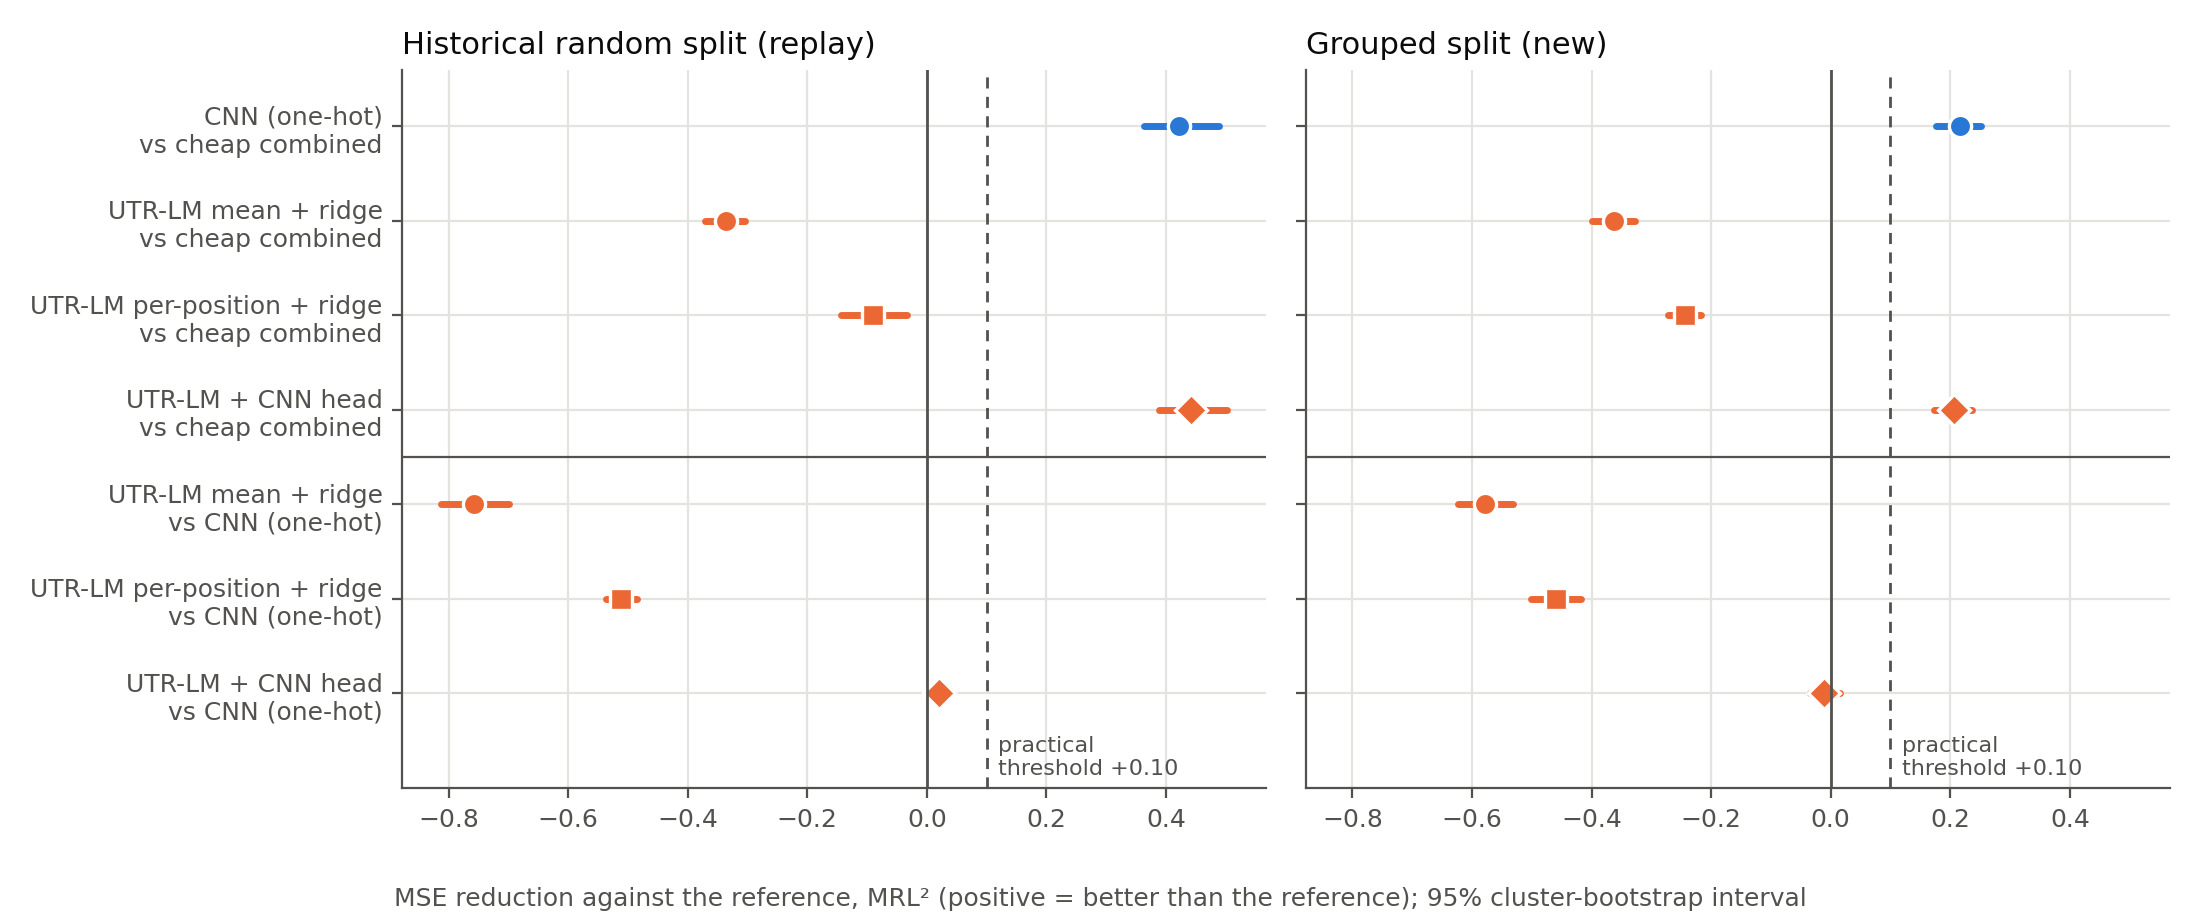
\includegraphics[width=\linewidth]{fig-paired-differences.png}
\caption{\textbf{MSE reduction against cheap combined (upper rows) and against the one-hot CNN (lower rows)}, with
95\% cluster-bootstrap intervals and the 0.10~MRL$^2$ threshold (dashed). Positive values favour the named method.
Source: original figure \m{article/assets/fig-paired-differences.png}, generated by the companion's
\m{make\_figures.py} from \m{run/metrics.json} (30 September 2026). (``historical'' in the figure panels and code is the random split.)}
\label{fig:paired}
\end{figure}

On the grouped split the whole interval for the CNN's MSE reduction lies above the 0.10 threshold, and its test MSE
across three seeds (0.559 to 0.570) does not change that verdict. For the top 150 picks the result differs. The
CNN's first 150 grouped-test picks held 86 high-MRL sequences against 83 for the cheap baseline, about 10 times the
chance rate for both. The gain of $+0.020$ [$-0.088$, $+0.132$] is not supported: this evidence cannot exclude a CNN
advantage of around 0.1 in precision, or a comparable disadvantage. The CNN's own precision ranged from 0.533 to
0.580 across seeds, wider than the observed difference. On the random split the CNN put 118 high-MRL sequences in
its first 150 against 87, a gain of $+0.207$ [$+0.124$, $+0.292$], the only supported precision gain over the reference
in either split.

Among the cheap baselines, every single feature set was worse than \m{cheap\_combined} on MSE on both splits; on
precision, 1--3-mer counts alone showed no supported difference from it (Appendix Table~\ref{tab:comparisons-all}).

\subsection{Frozen UTR-LM features gave no gain above the threshold over one-hot input}\label{sec:utrlm}
Ridge on UTR-LM embeddings was worse than ridge on cheap features on both splits, averaged or per position, and worse
than the one-hot CNN. As input to a CNN head, UTR-LM embeddings showed no supported difference from one-hot input on
the grouped split (MSE 0.570 against 0.560; $-0.010$ [$-0.034$, $+0.016$]). On the random split they were slightly
better on MSE ($+0.021$ [$+0.009$, $+0.034$], below the threshold) and worse on precision ($-0.127$ [$-0.179$,
$-0.023$]). On the grouped split, validation and test MSE ordered the two heads differently; neither ordering is
supported. Across seeds the UTR-LM CNN head's grouped test MSE ranged from 0.538 to 0.570 (Appendix
Table~\ref{tab:seeds}).

This says nothing about fine-tuning; in the authors' own ablation, under a different library and split, fine-tuning
outperformed a frozen model with an MLP head (Section~\ref{sec:background})~\citep{chu2024supp}.
mRNABench's saved results for this dataset~\citep{mrnabench_code} show the same ordering under a different protocol:
on its random split, a supervised CNN reached Pearson $r$ 0.862 (five seeds), a $k$-mer and GC ridge probe 0.788, a
probe on the excluded \m{utrlm-mrl} 0.649 and one on RiNALMo, another RNA language model, 0.821. On a harder
$k$-mer cluster split the $k$-mer and \m{utrlm-mrl} probes fell to 0.729 and 0.619. The probes used the full 855-nt
sequence; the CNN's input cannot be confirmed from the pinned code. This is context, not a replication or a verdict
on RNA foundation models.

\subsection{Accuracy cost minutes and gigabytes on a shared laptop}\label{sec:cost}
The whole run took \RunSeconds\,s (\RunMinutes{} minutes). The laptop was shared and swapping (about 7\,GB) during
the grouped fits, so these are single-run receipts, not a benchmark (Figure~\ref{fig:cost}; per-step times in
Appendix Table~\ref{tab:runlog}). Cheap combined ridge took 15 to 21\,s, mostly computing $k$-mer features, with the
alpha search included, using under 0.6\,GB. One CNN seed took 174 to 313\,s on the Apple GPU (Metal Performance
Shaders, MPS). The plotted seed-0 one-hot CNN took 205\,s (random) and 250\,s (grouped), with peak memory of 1.2 to
1.3\,GB. All three seeds together took 588\,s and 733\,s for the one-hot CNN, and 876\,s and 777\,s for the UTR-LM
CNN head (random, then grouped). On CPU (4 threads) one epoch took 151\,s against 11\,s on MPS in a pre-registration
probe, so no full CPU-only run was attempted. UTR-LM added a 4.87\,MB checkpoint, a \EmbedSeconds\,s CPU embedding
pass (\EmbedRSS\,GB peak), a \PosCacheGB\,GB embedding cache, and the run's largest memory step, 3.2\,GB for
per-position ridge.

\begin{figure}[!htbp]
\centering
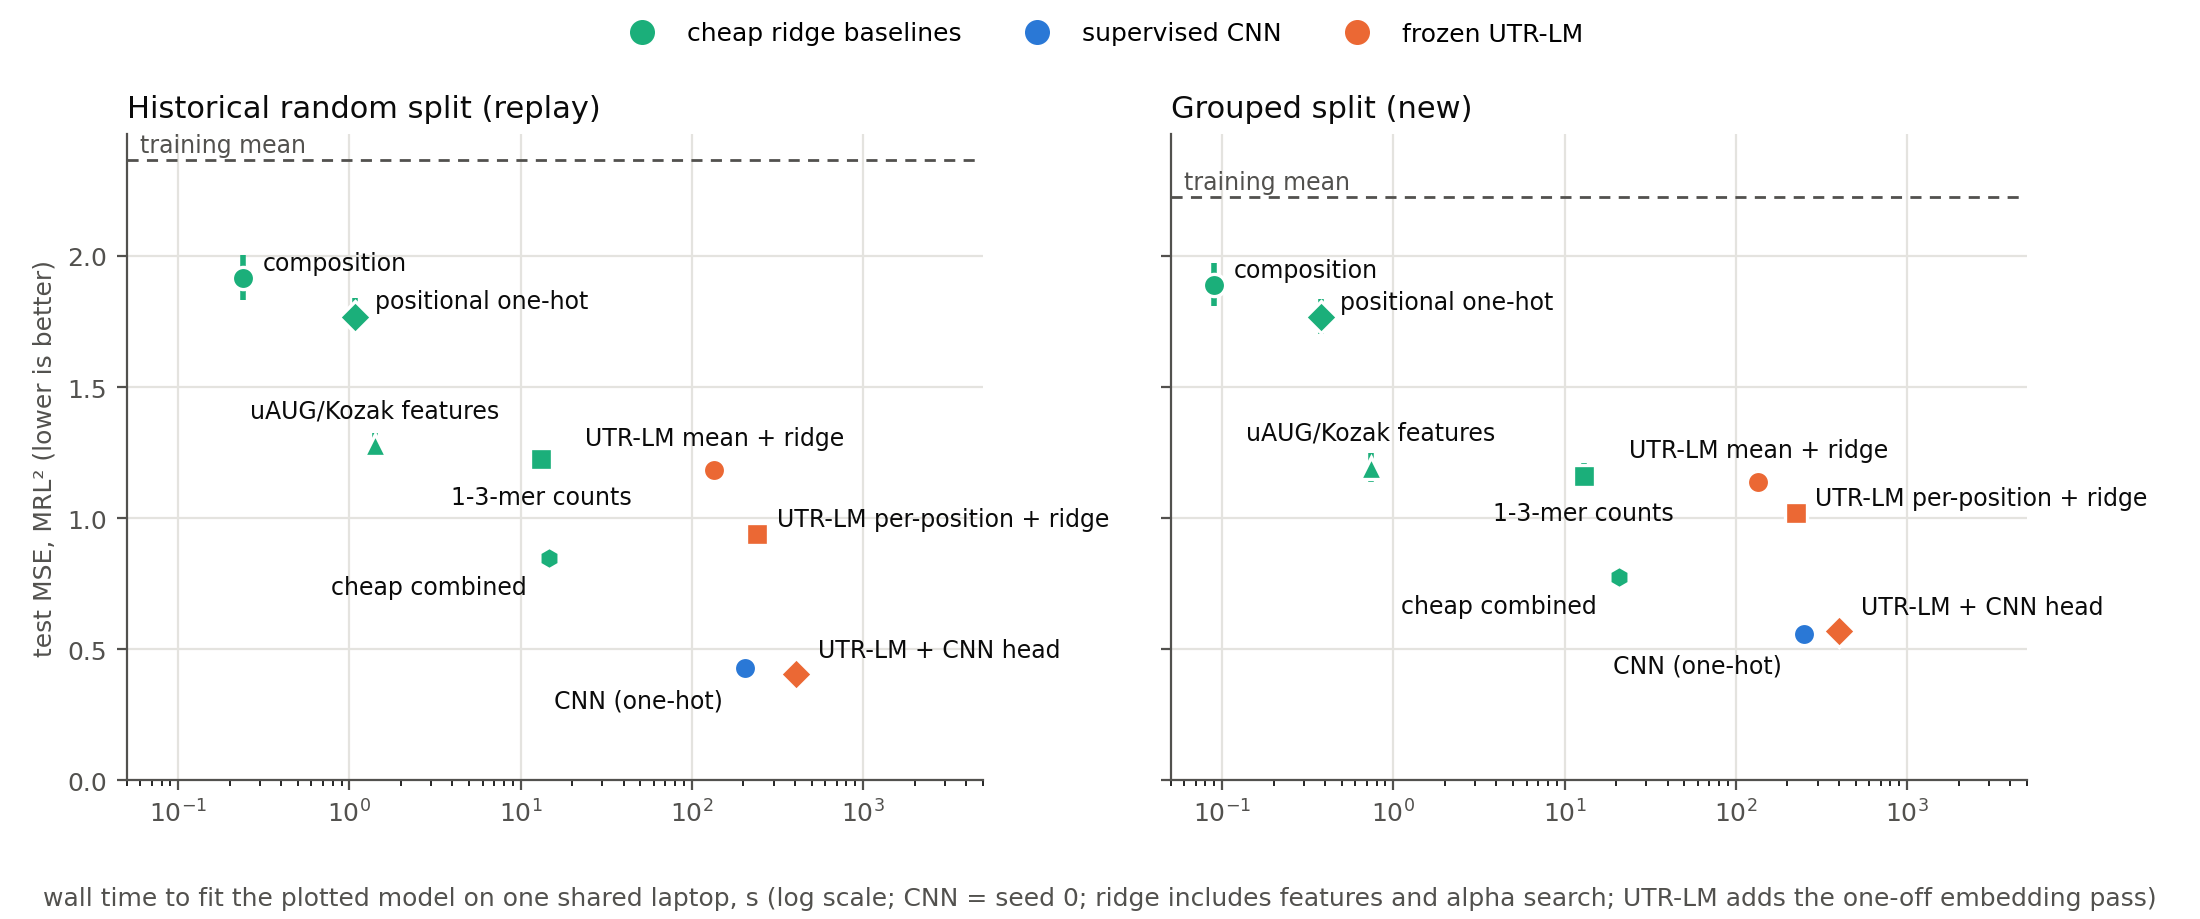
\includegraphics[width=\linewidth]{fig-accuracy-vs-cost.png}
\caption{\textbf{Test MSE (lower is better) against wall time to fit the plotted model}, log scale, random and grouped
splits side by side, with 95\% intervals. CNN points use the seed-0 time, ridge includes feature computation and the
alpha search, and UTR-LM adds the embedding pass. Single-run times on a shared laptop. Source: original figure
\m{article/assets/fig-accuracy-vs-cost.png} (companion run, 30 September 2026). (``historical'' in the figure panels and code is the random split.)}
\label{fig:cost}
\end{figure}

\subsection{Six declared examples show where the errors sit}\label{sec:examples}
The protocol fixed the example rule before test scoring: grouped-test records whose measured MRL is closest to the
10th, 50th and 90th percentiles; the record with the largest seed-0 CNN error; and the lowest-index SNV variant whose
reference is also in the test set (Table~\ref{tab:examples}). Every record shares one reporter context: the 25-nt
leader, the record's own 50-nt insert and the eGFP coding sequence.

\begin{table}[!htbp]
\centering
\scriptsize
\setlength{\tabcolsep}{2.5pt}
\caption{\textbf{Declared examples from the grouped test set}, with predictions from four methods (MRL). ``Index'' is
the source index; the 50-nt insert is printed beneath each row; \m{egfp\_poor\_performers} has no documented
definition. These six inserts are the only variable-region source
sequences embedded in the results archive, which also holds the constant 780-nt tail (Section~\ref{sec:availability}). Source: archived \m{run/metrics.json}, \m{splits.grouped.examples}.}
\label{tab:examples}
\begin{tabular}{@{}l l r r r r r r r@{}}
\toprule
Rule & Sub-library & Index & Reads & Measured & Cheap & CNN & UTR-LM & UTR-LM \\
 & & & & MRL & comb. & & + CNN & pos.\ ridge \\
\midrule
\inputtab{generated/tab_examples.tex}
\bottomrule
\end{tabular}
\end{table}

The 10th-percentile insert has an out-of-frame ATG at position 32; both CNN heads came within about 0.5 of the
measured 3.28, while both ridge models predicted above 5. The 90th-percentile insert has in-frame upstream ATGs at
positions 42 and 45. Every method underpredicted it; UTR-LM + CNN came closest (7.07 against 7.22). The largest CNN
error is a human UTR fragment measured at 1.99 and predicted at 6.70 to 8.10 by every method. It has no upstream ATG,
and ACC (a strong Kozak context) precedes the main AUG, so it carries none of the upstream-ATG or weak-Kozak features
known to lower loading. It had 328 reads, against a test median of 616. One record cannot show whether the low value
reflects biology the models miss or measurement noise. The SNV pair differs by one C$>$T change at insert position
24. Measured MRL rose by 0.66 (0.67 from the rounded values in Table~\ref{tab:examples}); the predicted changes were
$+0.17$ (cheap), $+0.07$ (CNN), $-0.06$ (UTR-LM + CNN) and $+0.32$ (UTR-LM ridge). Every method missed at least half of
the change, and one got its sign wrong.

\subsection{Errors concentrate at low read depth and in one trajectory family}\label{sec:errors}
\paragraph{Low read depth.} Grouped-split CNN MSE was 0.785 in the lowest read-depth quartile (100 to 315 reads) and
0.419 in the highest; for the cheap baseline, 1.024 and 0.606 (Figure~\ref{fig:errors}, right; Appendix
Table~\ref{tab:depth}). The \ErrOverTwo{} records with CNN errors above 2~MRL had a median of \ErrOverTwoReads{} reads
against \MedianReads{} overall. For their random library, Sample et al.\ note that low-read UTRs give noisier MRL;
with no replicate here, noise cannot be separated from model error. These are point estimates without intervals.

\paragraph{One trajectory family.} In \m{step\_worst\_to\_best\_allow\_uatg}, the only sub-library where the
grouped-split CNN's point estimate was worse than the cheap baseline's, its MSE was 1.134 against 0.405
(Figure~\ref{fig:errors}, left; Appendix Table~\ref{tab:perlib}). That sub-library has 210 grouped-test records in 5
families, the largest with 101 records. But 82\% of the CNN's squared error in that sub-library came from a different
family of 49 records (45 of them containing an ATG), where CNN MSE was 3.98 and the cheap baseline's 0.59. On the random
split the same sub-library, 744 test records in 38 families, showed the opposite (CNN 0.314, reference 0.723). This is
one family, not evidence that the CNN fails on uAUG designs, but an aggregate MSE can hide it. Check error by family.

\begin{figure}[!htbp]
\centering
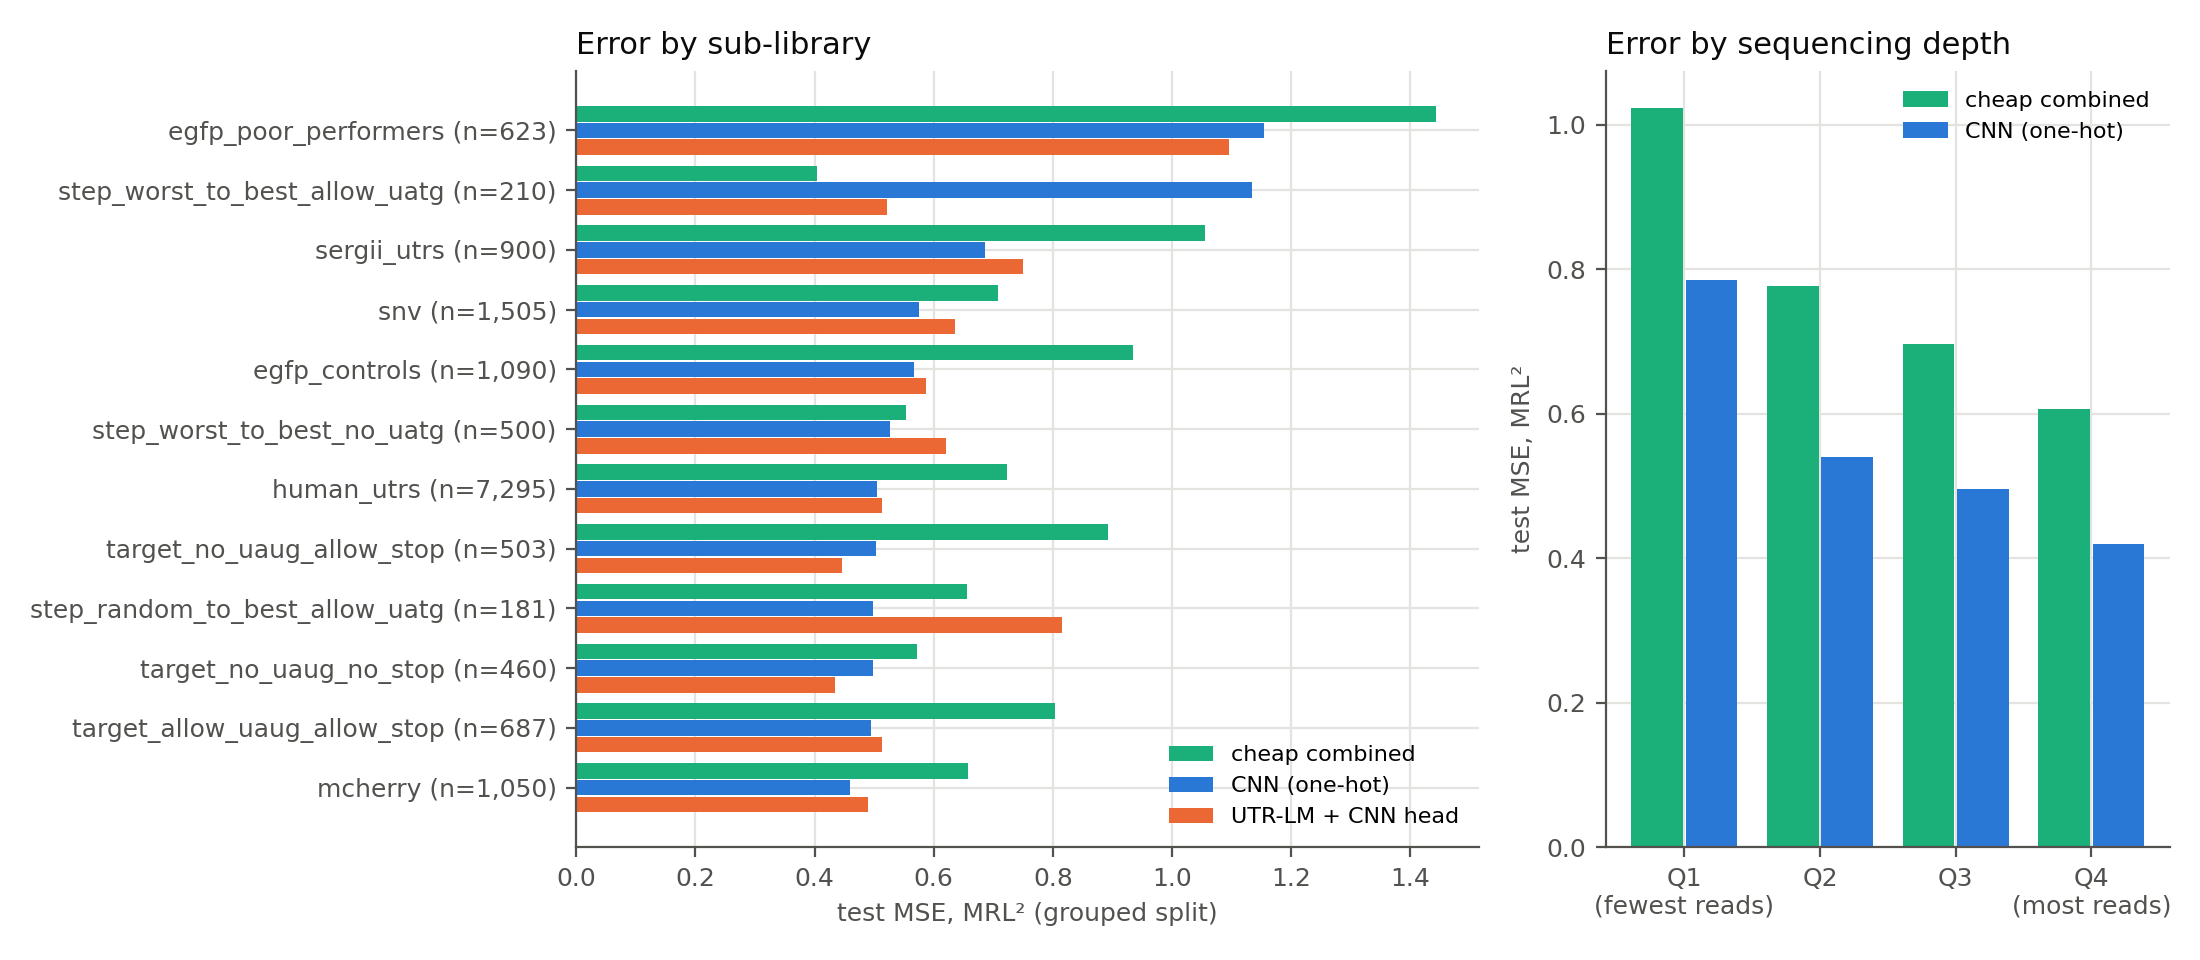
\includegraphics[width=\linewidth]{fig-error-by-library-and-depth.png}
\caption{\textbf{Grouped-split test MSE by sub-library (left) and by read-depth quartile (right).} Point estimates
without intervals; some sub-libraries have only five test families. Source: original figure
\m{article/assets/fig-error-by-library-and-depth.png} (companion run, 30 September 2026). (``historical'' in the figure panels and code is the random split.)}
\label{fig:errors}
\end{figure}

\subsection{Variant effects, split design and device choice}\label{sec:device}
\paragraph{Variant effects.} No method recovered the one SNV change in Table~\ref{tab:examples}, and this run does not
test variant-effect prediction. The original study reported $r^2$ 0.555 across 1,597 SNV pairs: a squared Pearson
correlation of log2 changes on high-read records, from a retrained model that had seen designed-library
sequences~\citep{sample2019}.

\paragraph{Split design.} Between the splits, the CNN's MSE advantage fell from $+0.422$ to $+0.216$~MRL$^2$ and its
precision advantage lost support; because overlap, composition and base rate all change, the drop cannot be attributed
to leakage alone.

\paragraph{Device divergence.} On this machine with torch 2.4.1, UTR-LM's final-layer output on Apple MPS differed from
CPU (maximum absolute difference 7.6 on 64 inserts), and masked-nucleotide accuracy on the first 1,000 inserts of the
data file fell from 0.412 to 0.335, about the share of the commonest base, with no error raised. All embeddings were
therefore computed on CPU; the cause was not found, and PyTorch's reproducibility notes~\citep{pytorch_repro} do not
promise CPU/GPU agreement. The CNNs trained on MPS after their untrained outputs matched CPU within
$1.1\times10^{-7}$, and after training their validation MSE on MPS and CPU agreed to within about $3\times10^{-8}$ for
all 12 fits (Appendix Table~\ref{tab:parity}). That is one metric on one setup, not general MPS parity; test predictions
were made on CPU. Users should compare CPU and accelerator outputs on their own setup before trusting them.

\subsection{Reproduction status}\label{sec:repro-status}
\noindent\fbox{\begin{minipage}{\dimexpr\linewidth-2\fboxsep-2\fboxrule\relax}\small
\textbf{Not yet reproduced under this repository's harness.} The values above are imported from the 30 September
2026 companion run; a same-machine clean-environment rerun repeated a subset (Appendix Table~\ref{tab:cleanroom}). No independent reproduction on other hardware has
been performed for this manuscript, and the repository's reproduction protocol has not been designed, approved or
executed.
\end{minipage}}

%======================================================================
\section{Discussion}\label{sec:discussion}
\subsection{The choice depends on what will be done with the predictions}
Table~\ref{tab:decision} and Appendix Figure~\ref{fig:flow} summarise the choice. For new families where MRL values
are needed, the grouped split supports the one-hot CNN. For a top-1\% pick list, it shows no supported difference
between the CNN and cheap combined ridge, so ridge is the cheaper choice, though the interval does not rule out a CNN
gain of around 0.1. For relatives of the training sequences, such as further steps of a design trajectory, the
random-split evidence applies and the CNN was better on both metrics. Frozen UTR-LM input gave no gain above the
prespecified threshold over one-hot input to the same CNN, so on this evidence its extra embedding step is not
justified. No supported difference is a finding, not a missing result, and not a demonstration of equivalence.

\begin{table}[H]
\centering
\scriptsize
\caption{\textbf{Decision summary.} P@150 is precision at 150. Grouped-split numbers unless stated; 95\%
cluster-bootstrap intervals; all results exploratory and measured with about 70,000 training labels.}
\label{tab:decision}
\begin{tabularx}{\linewidth}{@{}>{\raggedright\arraybackslash}p{2.6cm} L L L l@{}}
\toprule
Situation & What the evidence supports & Key numbers & Main caveat & Evidence \\
\midrule
New sequence families; MRL values needed & One-hot CNN & Grouped MSE 0.560 vs 0.776; reduction $+0.216$ [$+0.176$, $+0.252$] & Seed-0 model; one 49-record family failed badly & Tables~\ref{tab:methods}, \ref{tab:comparisons}; Fig.~\ref{fig:errors} \\
New sequence families; testing the top 1\% & No supported difference between the CNN and cheap combined ridge; ridge is cheaper & P@150 0.573 vs 0.553; gain $+0.020$ [$-0.088$, $+0.132$] & Interval allows a CNN gain of about 0.1 or a similar loss; CNN seeds spanned 0.533--0.580 & Table~\ref{tab:comparisons} \\
Candidates are close relatives of training sequences & One-hot CNN on both metrics & Random split: MSE $+0.422$ [$+0.363$, $+0.488$]; precision $+0.207$ [$+0.124$, $+0.292$] & 79.3\% of that test set has a relative in training; different test population & Table~\ref{tab:comparisons} \\
Considering frozen UTR-LM features & Not with a ridge head; with a CNN head, no supported difference from one-hot & Per-position ridge vs cheap $-0.244$ [$-0.272$, $-0.216$]; UTR-LM + CNN vs CNN $-0.010$ [$-0.034$, $+0.016$] & One checkpoint, frozen only & Table~\ref{tab:comparisons}; Fig.~\ref{fig:paired} \\
Only a CPU and seconds of fitting & Cheap combined ridge & 20.7\,s including alpha search; 0.45\,GB peak memory & Higher MSE than the CNN; times from a shared laptop & Table~\ref{tab:methods}; Fig.~\ref{fig:cost} \\
Single-variant effects needed & Nothing tested here & One declared SNV pair: measured $+0.66$, predicted $-0.06$ to $+0.32$ & One pair is an example, not an evaluation & Table~\ref{tab:examples} \\
Assay, cells, chemistry or label count differ & Outside the tested scope & -- & Run a grouped comparison on your own labels & Section~\ref{sec:limitations} \\
\bottomrule
\end{tabularx}
\end{table}

\subsection{What would change these conclusions}
A fresh cohort of new designs in the same assay would turn these exploratory numbers into a test, and a replicated
measurement would show how much of the remaining error is noise. A CNN precision gain at 150 with an interval above zero
would move the pick-list recommendation to the CNN. A learning curve at a few thousand labels would show whether the
ordering holds for small libraries. A fine-tuned UTR-LM, or another pretrained model, that beat the one-hot CNN by more
than 0.10~MRL$^2$ on a grouped split would reopen the case for foundation-model features on this assay.

%======================================================================
\section{Limitations}\label{sec:limitations}
\begin{itemize}
\item \textbf{Protein output or therapeutic effect.} MRL leaves out the ribosome-free mRNA fraction, so a high-MRL
sequence may still have a large untranslated fraction~\citep{castillohair2024}.
\item \textbf{Endogenous mRNAs.} MPRA-trained MRL models correlated only 0.11 to 0.25 with six endogenous translation
measurements in the main comparison of Karollus et al.~\citep{karollus2021} (Figure~\ref{fig:karollus}; their
Figure~7 splits it by UTR length and training set).
\item \textbf{Other reporters, cell lines or chemistries.} One eGFP reporter in HEK293T, one unreplicated run,
chemistry not stated.
\item \textbf{Few labels.} Every model trained on about 70,000 labels. No learning curve was measured, so nothing here
says a frozen model would do better with few labels.
\item \textbf{Variable-length UTRs.} Every insert is 50\,nt, and the CNN takes a fixed 50-nt input.
\item \textbf{Fine-tuned, larger or other foundation models.} One small frozen checkpoint was tested; Orthrus was
excluded for installation and scope reasons, not accuracy.
\item \textbf{Confirmatory claims.} Both test sets had prior exposure (the random test set was used for two published
controls; the grouped split was registered after viewing whole-dataset label summaries); every result is exploratory,
and the 22 comparisons are unadjusted.
\item \textbf{Uncertainty scope.} Cluster-bootstrap intervals describe sampling uncertainty for fixed models; training
seeds are reported separately and assay repeatability is not captured. Per-sub-library and read-depth analyses are
point estimates.
\item \textbf{Checkpoint provenance.} No sequence-overlap audit was run between the library and the UTR-LM pretraining
corpus.
\item \textbf{Platform.} All times and the exact-reproduction check come from one shared Apple M4 laptop; CNN training
used MPS; no cross-platform tolerance is established, and seeded CPU-only training was not tested for exact
repetition.
\item \textbf{Review.} Drafting, editorial review and fact checks of the original article were automated (Claude Opus);
the independent mechanical checks were run by another automated session (Codex). No human scientific review has taken
place.
\end{itemize}

\begin{figure}[!htbp]
\centering
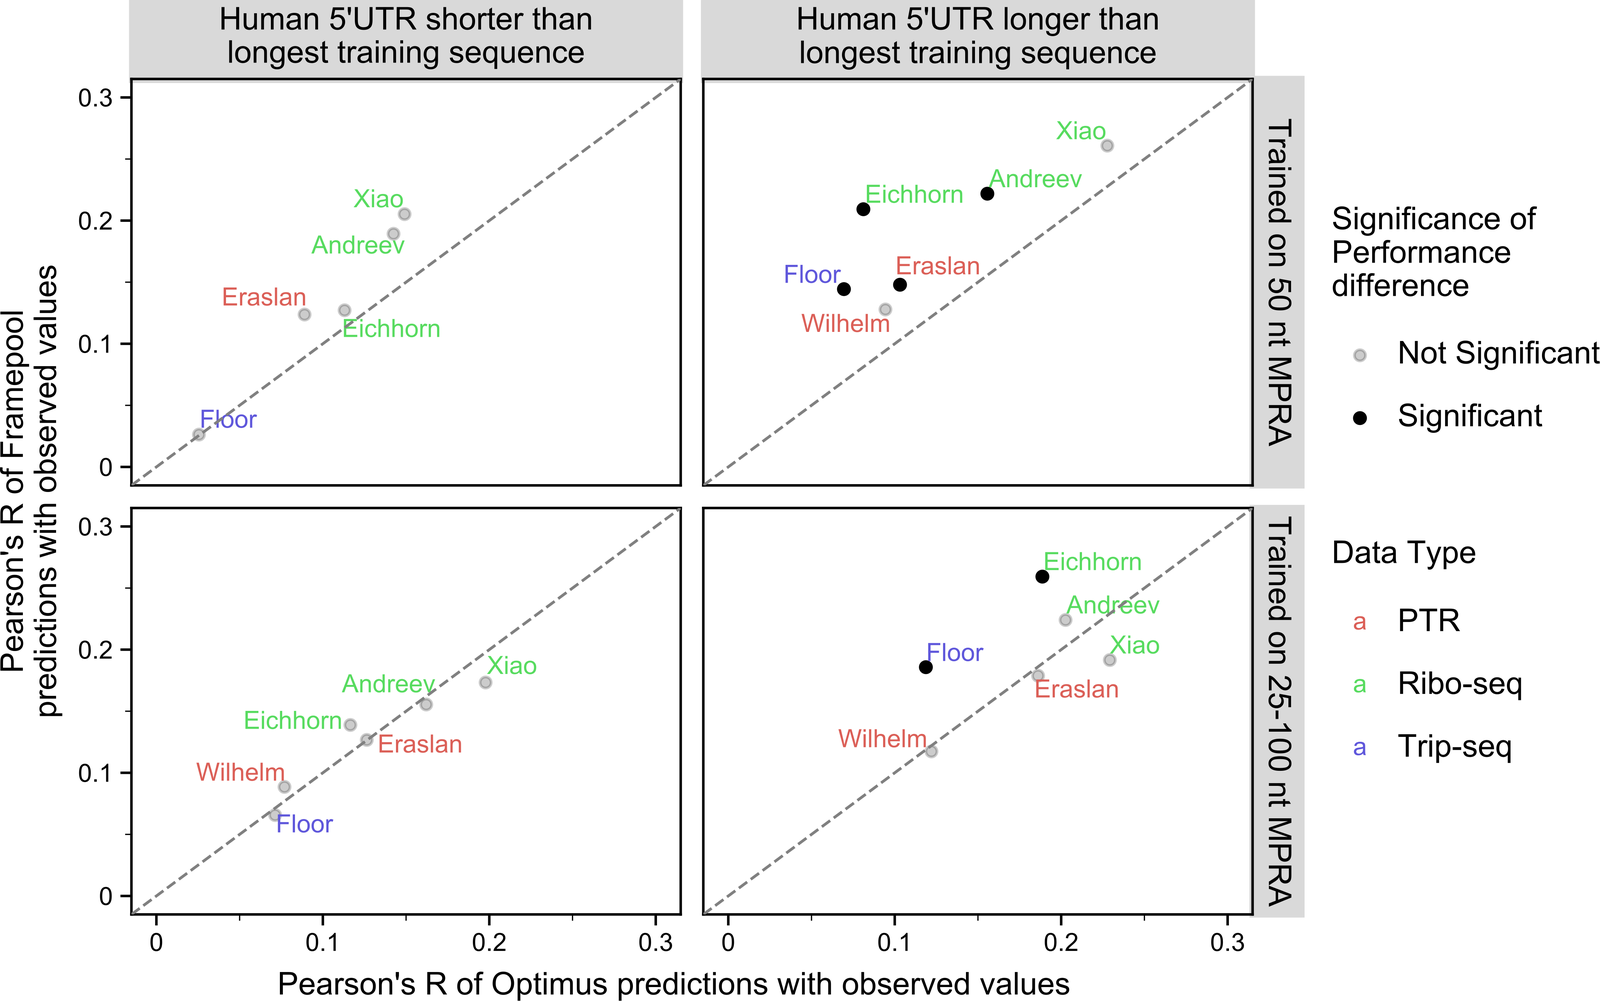
\includegraphics[width=0.75\linewidth]{10-karollus-fig4-endogenous-translation-transfer.png}
\caption{\textbf{MPRA-trained MRL predictions transfer poorly to endogenous translation.} Correlations of FramePool
against Optimus predictions with six endogenous translation datasets, all below about 0.26. From Karollus et al.\ 2021,
Fig.~4~\citep{karollus2021}, CC~BY~4.0.}
\label{fig:karollus}
\end{figure}

%======================================================================
\section{Data, code and licence availability}\label{sec:availability}
The study repository (\texttt{rewire-bio/utr-model-selection}) contains this manuscript and its build
(\texttt{make paper-imported}); the original article (\texttt{article/original.md} and the byte-identical
\texttt{article/published-original.md}, also embedded in this PDF as Supplement~S1); the companion code
(\texttt{companion/}, also as \texttt{downloads/utr-baselines.zip}, with the registered protocol in
\texttt{PROTOCOL.md}); and the results archive (\texttt{downloads/utr-baselines-results.zip}) with metrics, per-fit
receipts, predictions keyed by source index, verification outputs, device checks, the clean-environment rerun logs and
the independent automated checks (its \texttt{MANIFEST.md} lists the contents).

Neither archive contains the source datasets, model weights or embedding caches; they are downloaded at runtime from
pinned URLs and hash-checked. The results archive embeds only the six example inserts of Table~\ref{tab:examples} and
the constant 780-nt eGFP tail. The Hugging Face dataset card gives the processed data's licence as ``unknown'', so the
source records are not redistributed; the embedded excerpts are retained for auditability, and their redistribution
status is an open owner decision. Table~\ref{tab:examples} and Supplement~S1 reproduce these six records exactly as the
published article did and are subject to the same decision. GEO records are public; UTR-LM code and checkpoints are GPL-3.0 (its ESM files carry
Meta's MIT header); mRNABench code is AGPL-3.0. The licence of the companion code itself is to be set at publication.
The three reproduced literature figures are CC~BY~4.0 and are attributed in their captions.

%======================================================================
\section{AI assistance, review and disclosure}\label{sec:disclosure}
The original article's drafts, editorial reviews and fact checks were automated (Claude Opus). The independent
mechanical checks in the results archive were run by a separate automated orchestration session (Codex). The companion
code was run on the machine described. This manuscript was drafted by an AI model (Claude Opus,
\texttt{claude-opus-5-5}) from the archived evidence and reviewed by an independent AI reviewer instance of the same
model; the review and its disposition are recorded in \texttt{evidence/paper-migration/review.md} and
\texttt{review-disposition.md}. No human scientific review has taken place.

%======================================================================
\bibliographystyle{unsrtnat}
\bibliography{references}

%======================================================================
\clearpage
\appendix
\section{Reproducing the historical run}\label{app:repro}
The commands below are adapted from the original article (trailing comments moved to the text; one long command continued with a
backslash; the tutorial notebook, installed with \m{uv sync --extra test --extra notebook}, is omitted). They were run on 30 September 2026 and were \emph{not} re-executed for
this manuscript. They need uv~\citep{uv} and about 3\,GB of free disk (0.85\,GB environment, 31\,MB inputs, 1.3\,GB
embedding cache). \m{uv sync} installs the locked environment (Python 3.11, NumPy 1.26.4, scikit-learn 1.5.2, torch
2.4.1); the first \m{pytest} reported 10 passed and 1 skipped. The smoke run uses every 20th record (5,001), two CNN
epochs and seed 0; it is an installation check, not evidence. The full run took about 57 minutes on the Apple M4. Each
\m{verify.py} call ends with \m{ALL PASSED}, and the second \m{pytest} (with \m{UTR\_WORK} set) reported 11 passed.
\m{make\_figures.py} draws Figures~\ref{fig:paired}--\ref{fig:errors} from \m{metrics.json}; \m{describe\_failures.py} writes
\m{failures.json}, the source of the family, composition, device-parity and per-seed timing numbers.
\begin{lstlisting}
unzip utr-baselines.zip && cd utr-baselines
uv sync --extra test
uv run pytest -q

# Smoke run (installation check)
uv run python utr_baselines.py run-all --inputs runs/inputs \
    --work runs/smoke --smoke
uv run python verify.py --inputs runs/inputs --work runs/smoke

# Full run
uv run python utr_baselines.py run-all --inputs runs/inputs --work runs/full
uv run python verify.py --inputs runs/inputs --work runs/full
UTR_WORK=runs/full uv run pytest -q
uv run python make_figures.py --work runs/full --out runs/full/figures
uv run python describe_failures.py --work runs/full
\end{lstlisting}
The smoke run took 213\,s with CNN training on MPS, 199\,s in the clean rerun and 405\,s in a final check of the
published archive; with \m{--cpu-only} and \m{OMP\_NUM\_THREADS=4} it took 190\,s in an independent check, and
\m{verify.py} passed. A full \m{--cpu-only} run was not tested; at 151\,s per epoch it would take hours. The tutorial
notebook runs the smoke configuration and took 230\,s using MPS. \m{run-all} runs \m{fetch} (15 downloads, each checked
against a SHA-256 hash), \m{prepare} (constant leader and tail, exact GEO join, random-split hash \m{00e287b1\ldots}),
\m{embed}, one \m{fit} process per method and split, and \m{evaluate}. A rerun well outside the seed ranges in Appendix
Table~\ref{tab:seeds} (grouped one-hot CNN 0.559 to 0.570) is a reason to investigate, not an expected tolerance.

\paragraph{Rebuilding this manuscript.} \m{make paper-imported} runs \m{scripts/build\_paper.py} with the system Python
and local TeX Live. It verifies the archive and member digests, formats the tables in \m{paper/generated/}, converts
the original flowchart SVG with \m{rsvg-convert}, and runs pdflatex, BibTeX and pdflatex twice. It performs no
experiment, data download or environment creation. The receipt is \m{evidence/paper-migration/build-receipt.json}.

\section{The grouped split}\label{app:code}
Verbatim from lines 221--239 of \m{companion/utr\_baselines.py}; \m{GIANT\_FRACTION} is 0.01 and the seed is 20260930.
Components are built by linking records that share a GEO \m{mother} sequence or any identical 20-nt substring.
\lstinputlisting[language=Python,firstline=221,lastline=239]{../companion/utr_baselines.py}

\section{Supplementary tables}\label{app:supp}
All values are formatted from the archived results without recomputation.

\begin{table}[!tbp]
\centering
\scriptsize
\setlength{\tabcolsep}{3pt}
\caption{\textbf{All 22 registered paired comparisons.} Positive favours the named method over the reference. Source:
archived \m{run/metrics.json}, \m{splits.<split>.comparisons}.}
\label{tab:comparisons-all}
\stackedci
\begin{tabular}{@{}l >{\raggedright\arraybackslash}p{2.4cm} >{\raggedright\arraybackslash}p{1.5cm} l >{\raggedright\arraybackslash}p{1.8cm} l >{\raggedright\arraybackslash}p{1.8cm}@{}}
\toprule
Split & Method & Reference & MSE reduction [95\% CI] & Verdict & P@150 gain [95\% CI] & Verdict \\
\midrule
\inputtab{generated/tab_comparisons_all.tex}
\bottomrule
\end{tabular}
\end{table}

\begin{table}[H]
\centering
\scriptsize
\setlength{\tabcolsep}{3pt}
\caption{\textbf{Secondary metrics} (MAE in MRL; Pearson and Spearman correlations, undefined for the constant
predictor; enrichment = precision at 150 / test base rate; validation MSE; coverage), including the full-sequence
composition replay. Source: archived \m{run/metrics.json}.}
\label{tab:secondary}
\begin{tabular}{@{}l l r r r r r l@{}}
\toprule
Split & Method & MAE & Pearson & Spearman & Enrichment & Val.\ MSE & Coverage \\
\midrule
\inputtab{generated/tab_secondary.tex}
\bottomrule
\end{tabular}
\end{table}

\begin{table}[H]
\centering
\footnotesize
\caption{\textbf{Training-seed variability of the CNN heads}: test MSE / precision at 150 for each seed, and seconds per
seed. Paired intervals use seed 0, fixed in advance. Source: archived \m{run/metrics.json} (\m{per\_seed}) and
\m{run/failures.json} (\m{seconds\_this\_seed}).}
\label{tab:seeds}
\begin{tabular}{@{}l l l l l l@{}}
\toprule
Split & Head & Seed 0 & Seed 1 & Seed 2 & Seconds per seed \\
\midrule
\inputtab{generated/tab_seeds.tex}
\bottomrule
\end{tabular}
\end{table}

\begin{table}[H]
\centering
\footnotesize
\caption{\textbf{Test MSE by read-depth quartile} for the seed-0 CNN and the cheap-combined reference (quartile edges rounded to whole reads; point estimates,
no intervals). Source: archived \m{run/metrics.json} and \m{run/failures.json}.}
\label{tab:depth}
\begin{tabular}{@{}l l l r r@{}}
\toprule
Split & Quartile & Reads & CNN MSE & Reference MSE \\
\midrule
\inputtab{generated/tab_depth.tex}
\bottomrule
\end{tabular}
\end{table}

\begin{table}[H]
\centering
\scriptsize
\setlength{\tabcolsep}{3pt}
\caption{\textbf{Random and grouped test MSE by sub-library} for the reference, the seed-0 CNN and the UTR-LM CNN head
(point estimates; some grouped sub-libraries have only five test families). Source: archived \m{run/metrics.json},
\m{per\_library\_mse}.}
\label{tab:perlib}
\begin{tabular}{@{}l r r r r r r@{}}
\toprule
 & \multicolumn{3}{c}{Random split} & \multicolumn{3}{c}{Grouped split} \\
\cmidrule(lr){2-4}\cmidrule(lr){5-7}
Sub-library & Cheap comb. & CNN & UTR-LM + CNN & Cheap comb. & CNN & UTR-LM + CNN \\
\midrule
\inputtab{generated/tab_perlib.tex}
\bottomrule
\end{tabular}
\end{table}

\begin{table}[H]
\centering
\scriptsize
\setlength{\tabcolsep}{3pt}
\caption{\textbf{Library composition}: records per sub-library, their train/validation/test allocation and the number of
test-set families (components with at least one test record in that sub-library) under each split; families can span
sub-libraries, so these columns do not sum to the 9,640 / 6,002 test components. Source: archived \m{run/prepare.json} and \m{run/failures.json}.}
\label{tab:composition}
\begin{tabular}{@{}l r r r r r@{}}
\toprule
 & & \multicolumn{2}{c}{Random split} & \multicolumn{2}{c}{Grouped split} \\
\cmidrule(lr){3-4}\cmidrule(lr){5-6}
Sub-library & Records & Train/val/test & Test families & Train/val/test & Test families \\
\midrule
\inputtab{generated/tab_composition.tex}
\bottomrule
\end{tabular}
\end{table}

\begin{table}[H]
\centering
\scriptsize
\caption{\textbf{CNN device parity}: validation MSE computed on the training device and on CPU after training, for all
12 CNN fits. Agreement of one metric, not a general device-parity guarantee. Source: archived \m{run/failures.json},
\m{cnn\_device\_parity}.}
\label{tab:parity}
\begin{tabular}{@{}l l r l r r r@{}}
\toprule
Split & Head & Seed & Device & Val.\ MSE (device) & Val.\ MSE (CPU) & $|\Delta|$ \\
\midrule
\inputtab{generated/tab_parity.tex}
\bottomrule
\end{tabular}
\end{table}

\begin{table}[H]
\centering
\footnotesize
\caption{\textbf{Per-step process wall time} in the full run (seconds), from the archived \m{run/run-log.json}.
Ridge rows include process start-up and differ slightly from the in-process fit times in Table~\ref{tab:methods}; CNN rows
cover three seeds, whereas Table~\ref{tab:methods} gives seed 0 (in-process three-seed totals are in Section~\ref{sec:cost}). The steps sum to \StepSeconds\,s; the shell-measured whole run was
\RunSeconds\,s.}
\label{tab:runlog}
\begin{tabular}{@{}l r@{}}
\toprule
Step & Seconds \\
\midrule
\inputtab{generated/tab_runlog.tex}
\bottomrule
\end{tabular}
\end{table}

\begin{table}[H]
\centering
\footnotesize
\caption{\textbf{Independent mechanical checks} by \m{verify.py} (no shared code with the main script); check names are
verbatim from the archive, where ``historical'' is the random split. Source: archived
\m{run/verify.json}.}
\label{tab:verify}
\begin{tabularx}{\linewidth}{@{}L l L@{}}
\toprule
Check & Result & Detail \\
\midrule
\inputtab{generated/tab_verify.tex}
\bottomrule
\end{tabularx}
\end{table}

\begin{table}[H]
\centering
\footnotesize
\caption{\textbf{Clean-environment rerun on the same machine}: original and rerun test MSE and the maximum absolute
prediction difference. Source: \m{compare-with-original.json} in the archived \m{receipts/clean-room/}.}
\label{tab:cleanroom}
\begin{tabular}{@{}l l r r r@{}}
\toprule
Split & Method & Original MSE & Rerun MSE & Max $|\Delta|$ \\
\midrule
\inputtab{generated/tab_cleanroom.tex}
\bottomrule
\end{tabular}
\end{table}

\clearpage
\newgeometry{margin=1.1cm,headheight=14pt,includehead}
\section{Selection flowchart}\label{app:flow}
\begin{center}
\captionsetup{type=figure}
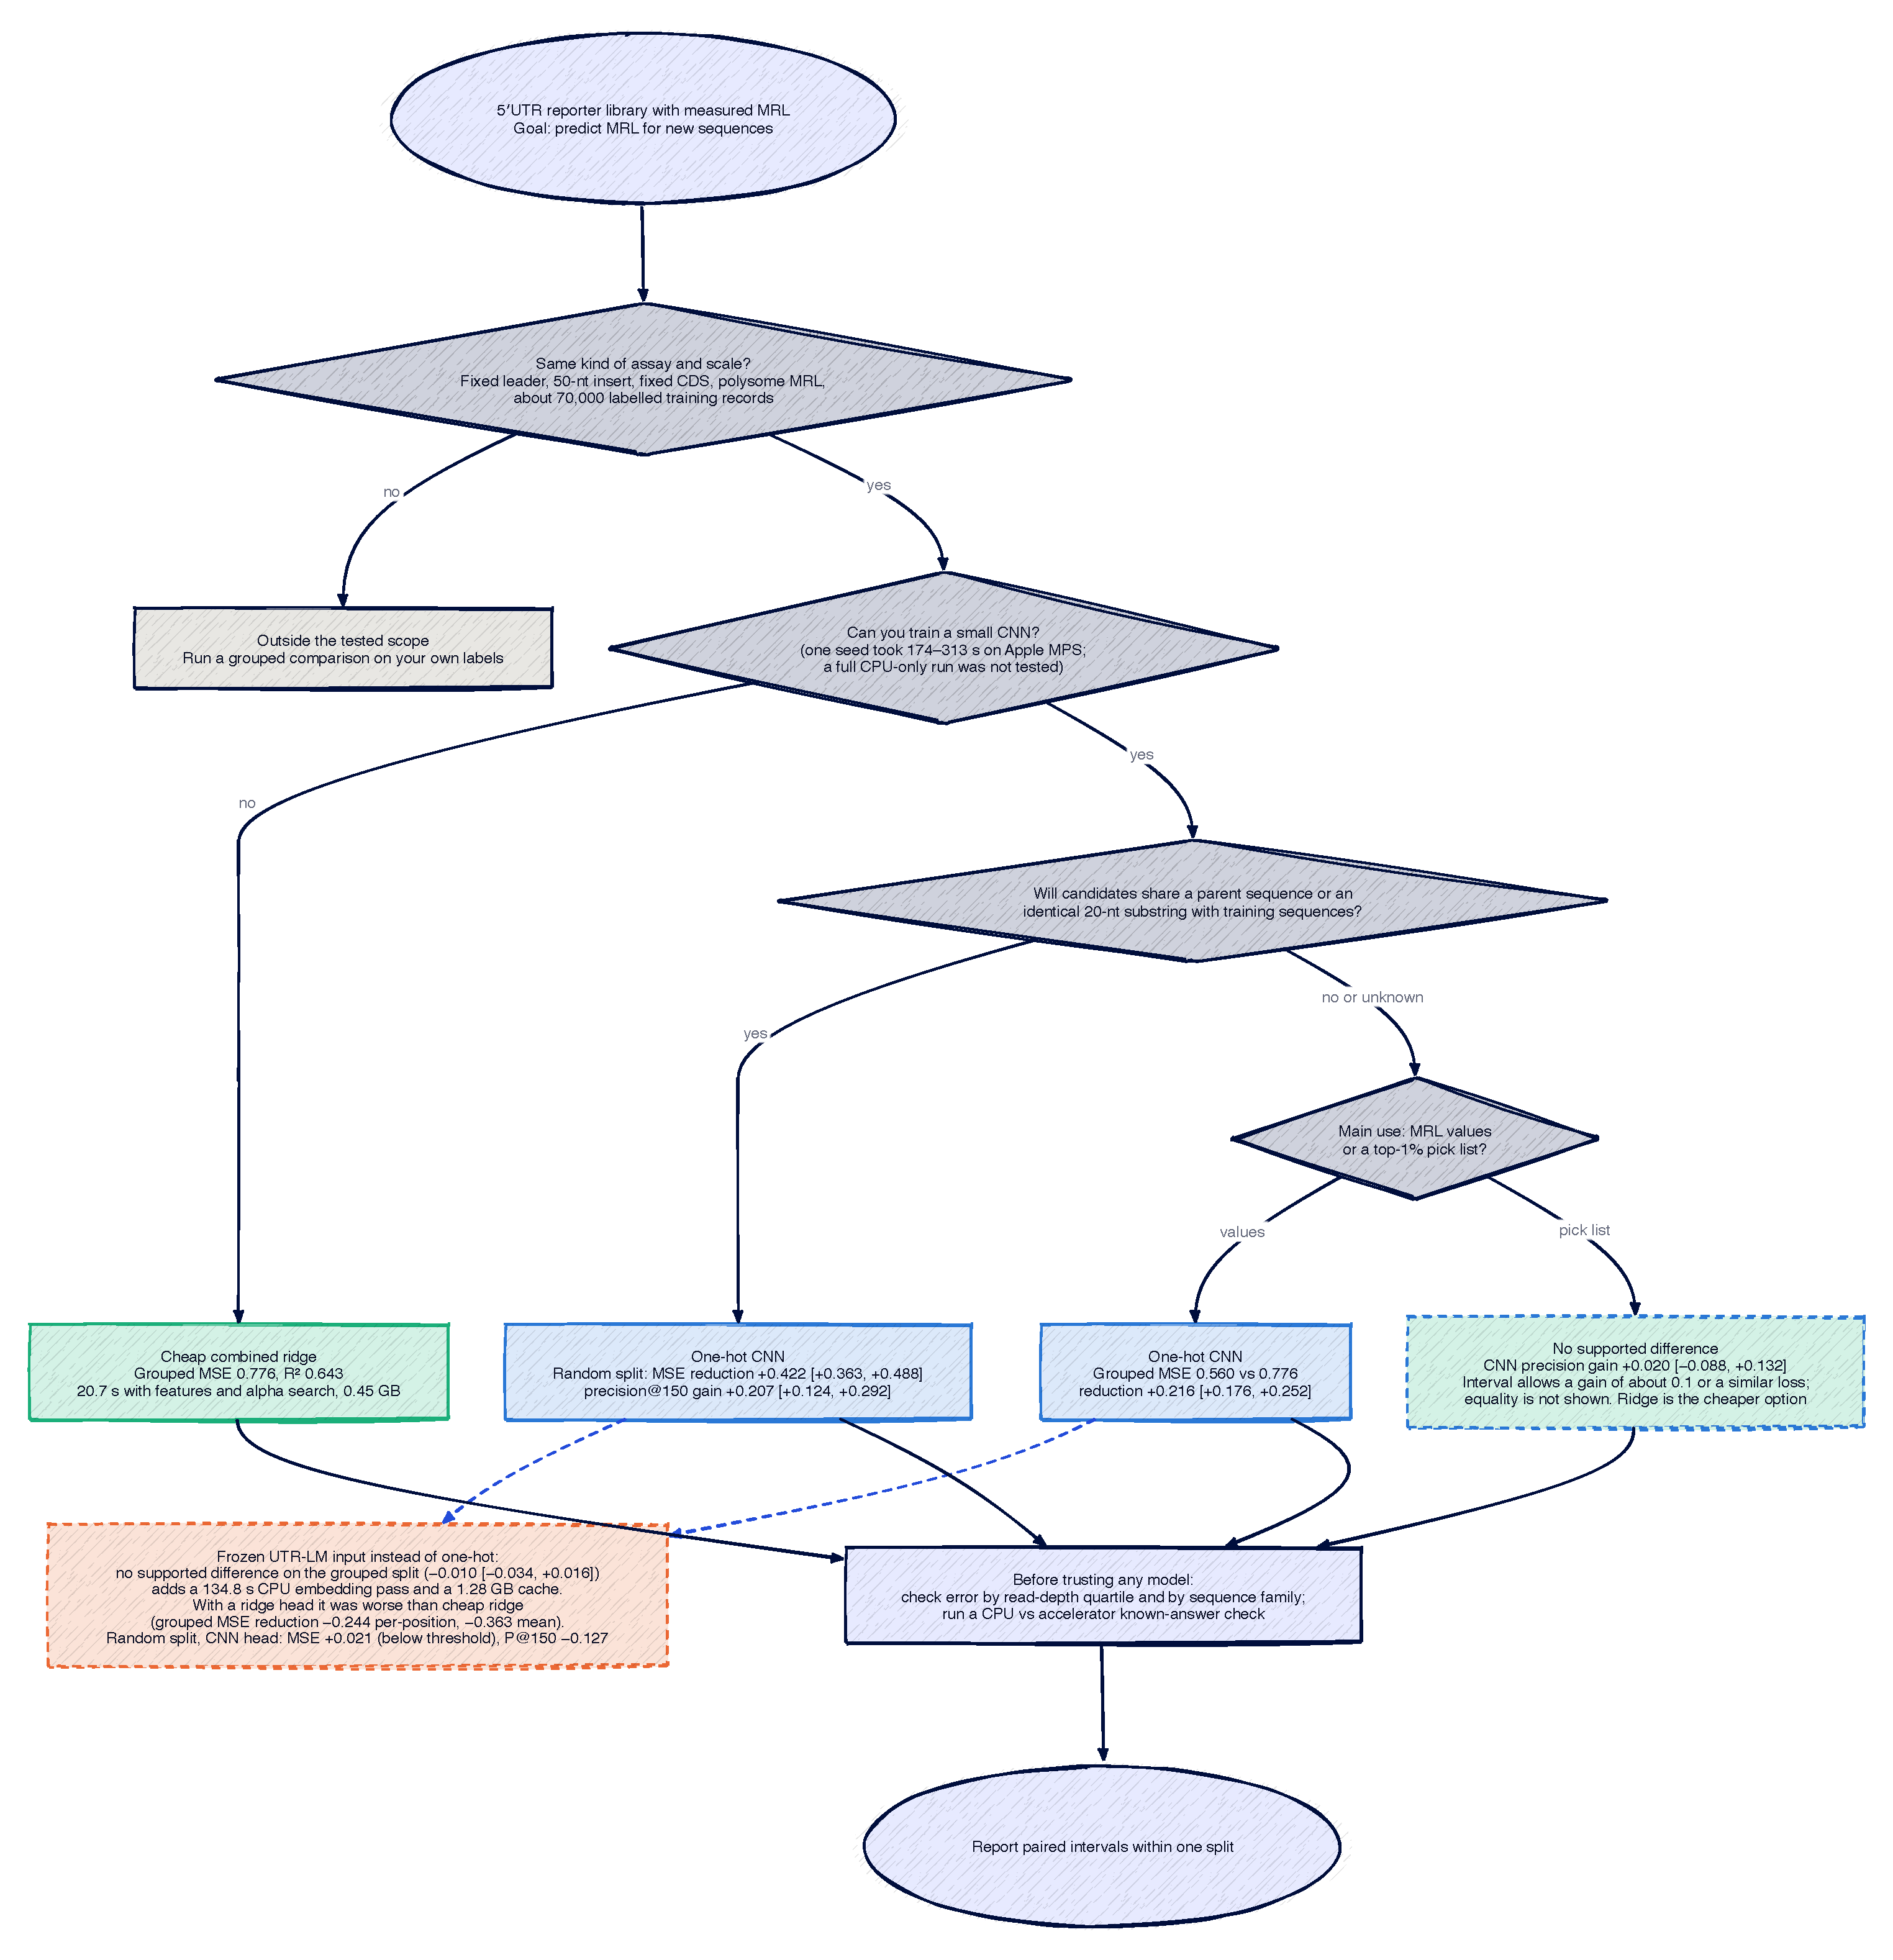
\includegraphics[width=\linewidth,height=0.80\textheight,keepaspectratio]{06-selection-flowchart.pdf}
\caption{\textbf{Selection flowchart} (original Figure~6, converted from \m{article/assets/06-selection-flowchart.svg};
D2 source in \m{06-selection-flowchart.d2}), built from the original Tables~1--3 (here Tables~\ref{tab:decision},
\ref{tab:methods} and \ref{tab:comparisons}). First check the assay and label scale are like this one; if a CNN cannot
be trained use cheap combined ridge; if candidates are relatives of training sequences, or MRL values are needed, use the
one-hot CNN; for a top-1\% pick list there is no supported difference and ridge is cheaper; frozen UTR-LM input is a side
note with no supported difference; all paths end with checks by read depth and family. The vector figure can be zoomed;
Table~\ref{tab:decision} gives the same routes in readable form.}
\label{fig:flow}
\end{center}
\restoregeometry

\section{Provenance, supplement and evidence mapping}\label{app:provenance}
\paragraph{Supplement S1 (original article).} The full original article, \emph{Choosing a Model for 5$'$UTR Translation
Experiments: Cheap Features, a Small CNN or Frozen UTR-LM} (30 September 2026), is retained unchanged in the repository
as \m{article/published-original.md} (byte-identical to the published source) and is embedded in this PDF as the
attachment \m{S1-published-original.md}. The repository copy \m{article/original.md} differs only in local links. Every
scientific result it reports appears in this manuscript; the section-by-section mapping is in
\m{evidence/paper-migration/content-coverage.md}.

\paragraph{Evidence ledger.} \m{evidence/paper-migration/claims-ledger.json} links each substantive claim to the
historical artifact (archive member or article text), a pointer inside it and its SHA-256. The results archive was read
in memory without extraction; its member digests are recorded in \m{evidence/migration-audit.json}. The table generator
(\m{scripts/paper\_extract.py}) stops the build if any generated value that also appears in the original article
differs from it: every cell of Tables~\ref{tab:methods} and~\ref{tab:comparisons} (including verdicts), the read-depth
and trajectory-family values, and the dependence, base-rate and resource numbers in the text. The recorded cross-check
found no difference. Values that the original did not print (the appendix tables) are formatted directly from the
digest-checked archive members.

\paragraph{Citation note.} Literature claims were checked for the original article in September 2026 and were not
re-retrieved during migration. DOIs for Sample et al., Chu et al.\ and mRNABench are those printed in the original
companion's \m{NOTICE.md}.

\end{document}
